
%%%
% Any line that begins with a percent symbol is a comment. To compile
% this document and view the output:
%
% Run Latex
% Run Bibtex
% Then run Latex twice.
%
% This should produce the output PDF file named main.pdf
%%%

% This defines the style to use for this document.
% Do not modify.
\documentclass[letterpaper]{article}

% The following are akin to "import" statements in Python or Java -
% these import useful commands into the document for you to use.  You
% don't have to modify any of these lines. The AAAI package formats
% this document in the style of submissions to the American
% Association for Artificial Intelligence conference, one of the top
% AI conferences in the world. You will find that many academic
% publications in AI use this format.
\usepackage{aaai}
\usepackage{times}
\usepackage{helvet}
\usepackage{courier}
\setlength{\pdfpagewidth}{8.5in}
\setlength{\pdfpageheight}{11in}
\usepackage{amsmath}
\usepackage{amsthm}
\usepackage{graphicx}
\usepackage{graphics}
\usepackage{moreverb}
\usepackage{subfigure}
\usepackage{epsfig}
\usepackage{txfonts}
\usepackage{algpseudocode}
\usepackage{multirow, multicol}
\usepackage{url}
\usepackage{tablefootnote}
\usepackage{color}

\setcounter{secnumdepth}{1}
\nocopyright

% Fill in your paper title, names and emails below
% The "\\" is used to break lines. The \url command
% is useful for typesetting URLs and email addresses (it uses the
% Courier font).
\title{Predicting the Quality of Wine}
 \author{Ethan Evans \and Calvin Spencer\\
 \url{{etevans, caspencer}@davidson.edu}\\
 Davidson College\\
 Davidson, NC 28035\\
 U.S.A.}

% This is the "true" start of the document. All the text in your
% write-up should be placed within the \begin{document} and
% \end{document} decorators.
\begin{document}

\maketitle % formats the title nicely, do not modify

% While at this point you could just begin your write-up, often, it's
% useful to write each section of your write-up in a separate tex
% file (not unlike the modular decomposition you do for code you
% write). These \input commands insert the contents of the
% specified tex files in the order specified. Every write-up you
% submit must contain the following sections, in the shown order. Open
% each of the indicated tex files to understand what goes in each
% section, as well as for more TeX tips.

% Place the contents of your abstract between the
% \begin{abstract} and \end{abstract} decorators.

\begin{abstract}

Wine preferences vary between consumers because of inherent differences in the human brain and palate. In this research, we aim to generate a regression model that can predict how a consumer will grade a wine based on physicochemical characteristics of the wine. While some of these properties have more importance to consumers’ ratings than others, it is difficult to derive a model that can accurately predict wine ratings using multivariate analysis. Despite this difficulty, there is a distinct difference between the prediction accuracy on red wines versus white wines. It is clear that more research and experimentation should be done before deploying an algorithm like this to the industrial world, with which its impacts will be commensurate with its accuracy.

% The \textbf{} command makes the specified text bold. The \emph{} or
% \textit{} command are used to italicize text. In general, text is never
% underlined.

% DON'T FORGET TO MATCH EACH OPEN BRACE WITH A CLOSING BRACE!
\end{abstract}



% The \section{} command formats and sets the title of this
% section. We'll deal with labels later.
\section{Introduction}
\label{sec:intro}

Wine tasting has been a tradition of wine enthusiasts for centuries. Each taster evaluates the quality of the wine based on their own unique palate and generates consumer preferences. The process of rating wines is thought to be completely subjective, but what if one could predict how a particular wine is rated based on physicochemical characteristics of the wine like alcohol content and acidity. Employing this technique would revolutionize the wine consumer market through the creation of new wines and targeted advertising of certain wines. \\\\
An idea like that of predicting wine quality based on its characteristics becomes feasible when taking a regression modeling approach. Regression analysis will consider both the characteristics and ratings of pre-existing wines and use patterns in that data to rate wines that the model has not seen yet. Through this type of modeling, we can ideally rate any kind of wine both in existence and in imagination. In this paper, we followed this regression approach to see if we could accurately predict a subjective wine rating from objective inherent characteristics and previous ratings. \\\\
The data used to fuel our regression model came from the UCI Machine Learning Repository, created by Paulo Cortez, Antonio Cerdeira, Fernando Almeida, Telmo Matos, and Jose Reis. Data was split into two sets, one set contained data on the Portuguese "Vinho Verde" red wine variant and the other on the corresponding white wine variant. The following are the eleven physicochemical variables that were recorded for each wine: fixed acidity, volatile acidity, citric acid, residual sugar, chlorides, free sulfur dioxide, total sulfur dioxide, density, pH, sulphates, and alcohol. In addition, wine experts graded each wine on a scale of 0 to 10 with 0 representing “very bad” and 10 representing “very excellent.” The median of three experts’ grades was compiled as this variable. The red wine dataset contains 1,599 wines, and the white wine dataset contains 4,898 wines. \\\\
In this paper, we will detail the process of exploring the data, augmenting the data, generating and optimizing regression models for both red and white wines, and comparing the models’ effectiveness.
\\

% Citations: As you can see above, you create a citation by using the
% \cite{} command. Inside the braces, you provide a "key" that is
% uniue to the paper/book/resource you are citing. How do you
% associate a key with a specific paper? You do so in a separate bib
% file --- for this document, the bib file is called
% project1.bib. Open that file to continue reading...

% Note that merely hitting the "return" key will not start a new line
% in LaTeX. To break a line, you need to end it with \\. To begin a 
% new paragraph, end a line with \\, leave a blank
% line, and then start the next line (like in this example).



\section{Data Preparation}
\label{sec:background}

The following data preparation and preprocessing steps were completed independently and identically in both the red wine and white wine data sets. All experimental methodologies and data manipulation was completed using auxiliary Python libraries including \textit{scikit-learn}, \textit{numpy}, \textit{pandas}, and \textit{matplotlib}. The data was first shuffled, and one-fifth of it was held out for a final testing set. The remaining 80\% of the data was used for training our regression models. \\\\
We plotted individual features against the wine quality to visualize if there were any apparent relationships between them (seen below). As we expected, this varied depending on which feature was chosen. Some features in the red wine dataset, such as alcohol and volatile acidity, showed a directional preference as wine quality increased. This indicated that indeed, some features appear to correlate with a higher quality wine. For others, such as residual sugar, there was no obvious correlation between the feature and the wine quality. \\\\
\begin{figure}[htb]

  \centering  % centers the image in the column

  % replace the second argument below with your filename. I like to
  % place all my figures in a sub-directory to keep things organized
  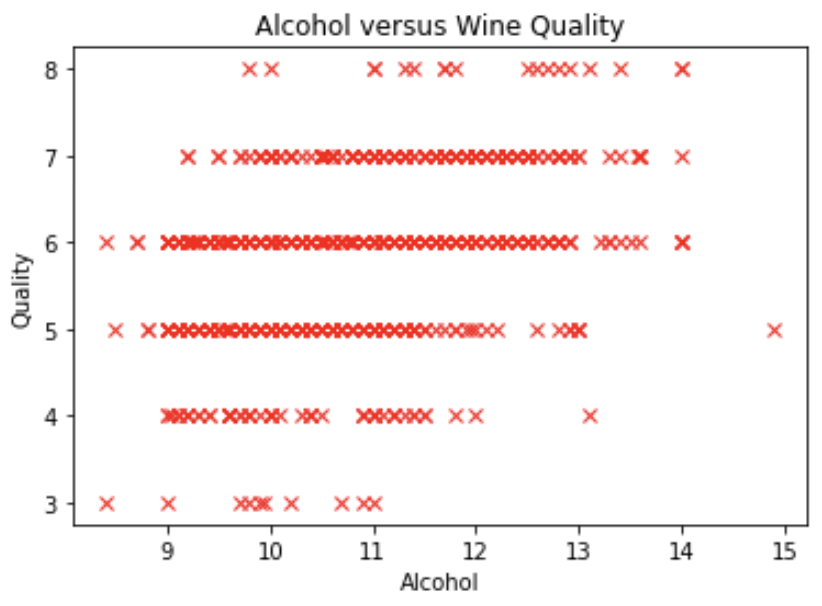
\includegraphics[width=\linewidth]{template/figs/alcohol.png}

  % *Every* figure should have a descriptive caption.
  \caption{This distribution of wine qualities and their alcohol content indicates a slight positive correlation between the two variables.}

  % The label is a handle you create so that you can refer to this
  % figure (using the \ref{} command) from other parts of your
  % document. LaTeX automatically renumbers figures and updates
  % references when you recompile, so you should do it this way rather
  % than hard-coding in references. Notice that I've also been
  % creating labels for the various sections in the document; I could
  % use \ref{} command to refer to those sections using their labels
  % too.
  \label{fig:alcohol}

\end{figure}

\begin{figure}[htb]

  \centering  % centers the image in the column

  % replace the second argument below with your filename. I like to
  % place all my figures in a sub-directory to keep things organized
  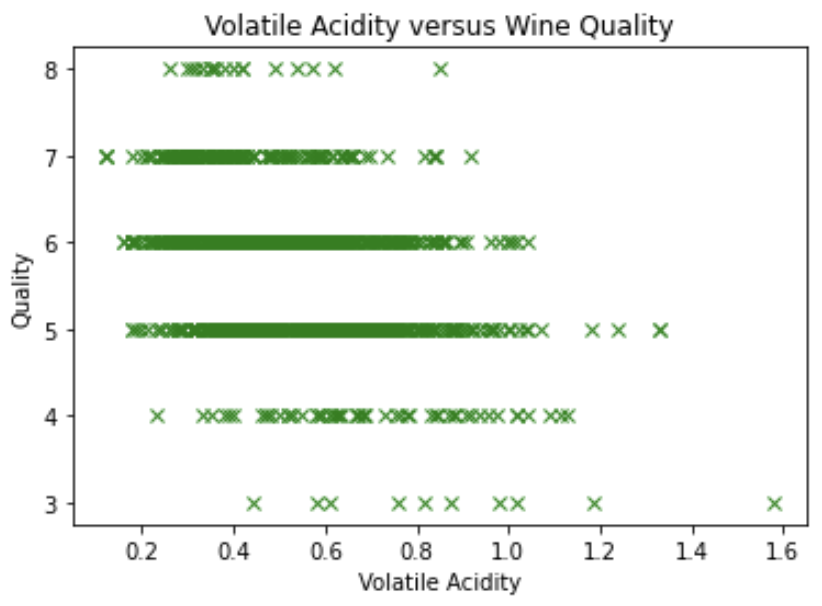
\includegraphics[width=\linewidth]{template/figs/acidity.png}

  % *Every* figure should have a descriptive caption.
  \caption{This distribution of wine qualities and their volatile acidity indicates a slight negative correlation between the two variables.}

  % The label is a handle you create so that you can refer to this
  % figure (using the \ref{} command) from other parts of your
  % document. LaTeX automatically renumbers figures and updates
  % references when you recompile, so you should do it this way rather
  % than hard-coding in references. Notice that I've also been
  % creating labels for the various sections in the document; I could
  % use \ref{} command to refer to those sections using their labels
  % too.
  \label{fig:acidity}

\end{figure}

\begin{figure}[htb]

  \centering  % centers the image in the column

  % replace the second argument below with your filename. I like to
  % place all my figures in a sub-directory to keep things organized
  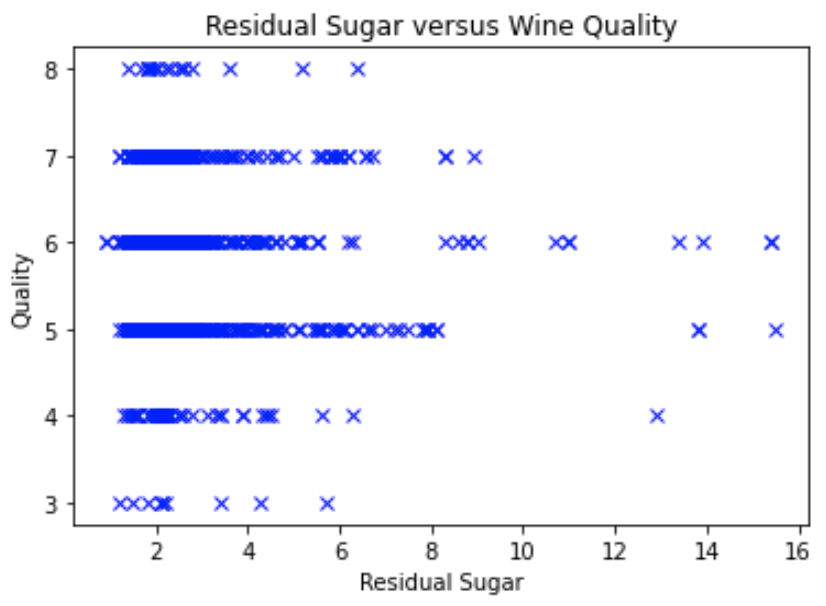
\includegraphics[width=\linewidth]{template/figs/sugar.png}

  % *Every* figure should have a descriptive caption.
  \caption{There is no strong correlation between wine quality and residual sugar.}

  % The label is a handle you create so that you can refer to this
  % figure (using the \ref{} command) from other parts of your
  % document. LaTeX automatically renumbers figures and updates
  % references when you recompile, so you should do it this way rather
  % than hard-coding in references. Notice that I've also been
  % creating labels for the various sections in the document; I could
  % use \ref{} command to refer to those sections using their labels
  % too.
  \label{fig:sugar}

\end{figure}
This exploratory phase of our experiment was crucial to the implementation of our solution. These findings indicated some features might be more correlated than others, and led us to consider using a specific type of regression which focuses on reducing the impact of unrelated variables on our model. \\\\
The eleven input features of the dataset were then scaled using standardization. This transforms the data into a normal distribution feature-wise, which will allow the regression solver to more efficiently converge on a solution. More on this can be found in Scikit-Learn’s data preprocessing user guide \cite{sklearn_api}. \\\\
With all of this background information, we made several key choices with our regression models that allow for the more efficient and accurate prediction model. \\\\

\section{Experiments}
\label{sec:expts}

\begin{figure*}[htb]

  \centering  % centers the image in the column

  % replace the second argument below with your filename. I like to
  % place all my figures in a sub-directory to keep things organized
  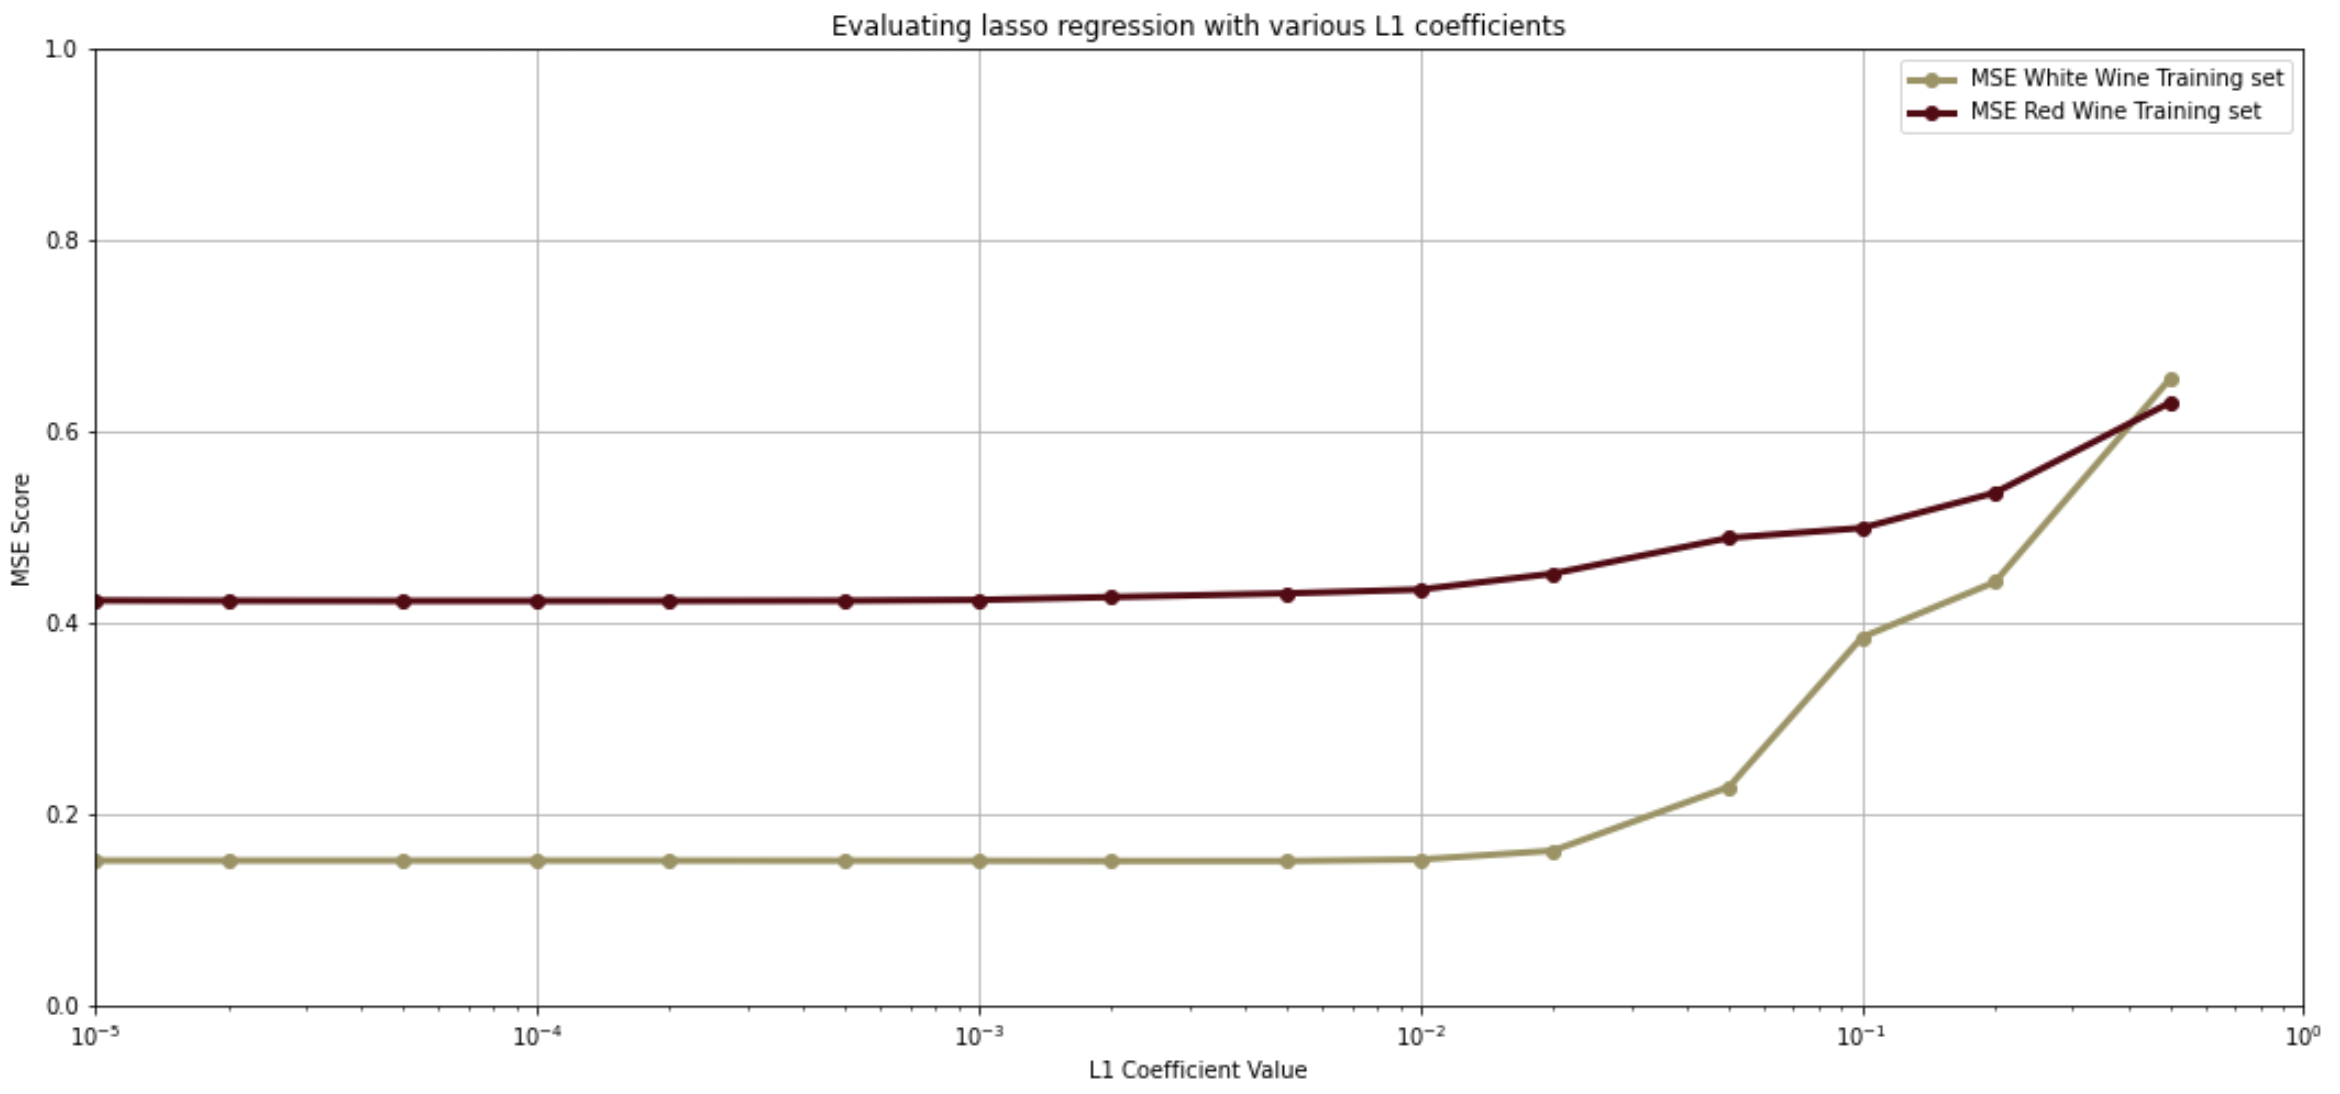
\includegraphics[width=\linewidth]{figs/hptuning.png}

  % *Every* figure should have a descriptive caption.
  \caption{Mean squared error (MSE) by L1 regularization coefficient value for both the red and white wine training sets. The optimal L1 coefficient for the red wine dataset is at 0.00012 with an MSE of 0.424. The optimal L1 coefficient for the white wine dataset is at 0.0024 with an MSE of 0.152. Dark red indicates the red wine dataset, and beige indicates the white wine dataset.}

  % The label is a handle you create so that you can refer to this
  % figure (using the \ref{} command) from other parts of your
  % document. LaTeX automatically renumbers figures and updates
  % references when you recompile, so you should do it this way rather
  % than hard-coding in references. Notice that I've also been
  % creating labels for the various sections in the document; I could
  % use \ref{} command to refer to those sections using their labels
  % too.
  \label{fig:hptuning}

\end{figure*}

We approached this regression problem knowing that we wanted to employ regularization methods in some manner. Regularization simplifies the model by tuning the weights of certain features, and thus reducing the potential for overfitting. Our initial thought was to implement lasso regression, which is particularly successful in multivariate models where some features may play a larger role in predicting the outcome than others. If you visualize each feature holding some weight or coefficient value, lasso regression shrinks these weights all the way to zero on less important features through a process called L1 regularization. Therefore, due to our prior data exploration process, we hypothesized that some variables would have stronger correlations with wine rating than others, so feature selection was an important consideration for our choice of model. \\\\
We compared this to another common regression technique known as ridge regression which implements a slightly different regularization method that shrinks weights but doesn’t set them to zero. The weights of features in ridge regression never reached zero, while they often did in our lasso models, which match the proper functionalities of the two types of regression. Despite converging on different L1 regularization coefficients, the mean squared error of each type of regression was comparable and did not indicate a strong difference in their coefficients of determination. However, we decided to move forward with the lasso approach due to what we know about its built-in feature selector properties. \\\\
After settling on lasso regression, we turned to the Lasso structure as a part of \textit{scikit-learn}’s linear modeling package. Lasso regression adopts coordinate descent as its optimizer and tunes learning rate automatically. We performed 5-fold cross validation on our training data, using mean squared error as our scoring metric. In terms of hyperparameters in question, our main focus was on optimizing the L1 regularization coefficient. This would determine the degree at which certain features were rejected from the model. We tuned this value through built-in grid search functionality to optimize the mean squared error of the model (seen in figure~\ref{fig:hptuning}). \\\\
For the red wine dataset, the mean squared error over the 5-fold cross validation data was 0.424 and the optimal L1 coefficient was 0.00012. For the white wine dataset, the mean squared error was 0.152 and the optimal L1 coefficient was 0.0024. After finding the ideal L1 coefficient, we fit our models to the training and test datasets and evaluated them by the coefficient of determination. \\\\

\section{Results}
\label{sec:results}

We fit our two models for red wine and white wine using their respective optimal hyperparameters and found distinct differences between the two types of wine. As for the red wine, the training dataset had a coefficient of determination of 36.56, and the test dataset had a coefficient of determination of 35.06. For the white wine, the training dataset had a coefficient of determination of 27.87, and the test dataset had a coefficient of determination of 28.51. This is tabulated in figure~\ref{tab:example}. In addition, as seen in figure~\ref{fig:hptuning} above, the white wine dataset had a lower mean squared error than the red wine dataset. \\\\

\begin{figure}[htb]
  \centering
  \begin{tabular}{|c|c|c|} 
    \hline
     & Red Wine & White Wine \\
    \hline
    Training Set & $36.56$ & $27.87$ \\
    Test Set & $35.06$ & $28.51$\\
    \hline
  \end{tabular}

  % As with figures, *every* table should have a descriptive caption
  % and a label for ease of reference.
  \caption{Coefficient of determination ($R^2$) values for both the training and test sets for red and white wine.}
  \label{tab:example}

\end{figure}

This indicates that our model for red wines fit the data slightly better than the model for white wines. One of the biggest differences between the red and white wine datasets (other than the inherent physicochemical differences in the wine) was the size of the dataset. The white wine dataset was roughly three times larger than the red wine dataset, which meant that it trained on far more data. Perhaps we did not address overfitting as dutifully, which may explain the lower mean squared error and coefficient of determination. In terms of the choice of regression model, the minor difference between lasso and ridge regression may indicate the need for further research and experimentation with these models and data. \\\\
In addition, the optimized feature coefficients differed between red and white wine data. Values for each coefficient for both datasets is tabulated in figure~\ref{tab:coeff}. A lot of the features were weighted similarly between the two types of wine such as residual sugar, free sulfur dioxide, total sulfur dioxide, and density. However, other features like chlorides are drastically different impacts on their respective regression models, indicating chlorides in red wine may be more influential to the overall wine quality.


\begin{figure*}[htb]

  \begin{tabular}{|c|c|c|c|c|c|c|} 
    \hline
     & Fixed Acidity & Volatile Acidity & Citric Acid & Residual Sugar & Chlorides & Free Sulfur Dioxide\\
    \hline
    Red Wine & $-.016$ & $-0.890$ & $0.227$ & $0.024$ & $-2.176$ & $0$\\
    White Wine & $-0.023$ & $-1.319$ &  $0$ & $0.023$ & $0$ & $0.009$ \\
    \hline
  \end{tabular}
 \\\\\\\
\begin{tabular}{|c|c|c|c|c|c|} 
    \hline
     & Total Sulfur Dioxide & Density & pH & Sulphates & Alcohol\\
    \hline
    Red Wine & $-0.003$ & $0$ & $-0.450$ & $0.926$ & $0.261$\\
    White Wine & $-0.003$ & $0$ & $0$ & $0.496$ & $0.357$ \\
    \hline
 \end{tabular}

  % As with figures, *every* table should have a descriptive caption
  % and a label for ease of reference.
  \caption{Features and their given weights assigned by the regression model for both red and white wine.}
  \label{tab:coeff}

\end{figure*}

%    Red Wine & $-.016$ & $-0.890$ & $0.227$ & $0.024$ & $-2.176$ & $0$ & $-0.003$ & $0$ & $-0.450$ & $0.926$  $0.261$\\
%White Wine & $-0.023$ & $-1.319$ &  $0$ & $0.023$ & $0$ & $0.009$ & $-0.003$ & $0$ & $0$ & $0.496$ & $0.357$ \\

\section{Broader Impacts}
\label{sec:impacts}

What this model offers the wine industry is a mathematical understanding of the relationships between wine features and rating. People can describe the qualitative features they experience when tasting a wine, but implementing a model such as this provides an opportunity to carry out this type of testing at a faster rate. Additionally, the model that is generated can provide valuable insights into how humans’ rate wine. Individuals could identify through our model which traits affect the rating the greatest. Wineries can profit off this information by adjusting their recipes using this data generated by regressing these data sets. \\\\
Despite the automation that machine learning algorithms provide, the implementation and design of these methods depend upon human decision making. Implicit bias that the developer or data source may possess can cause an algorithm to behave improperly, resulting in inaccurate predictions \cite{mehrabi2019survey}. By the same token, these biases can worsen inequalities if a machine learning model is rooted in logic that negatively scores specific racial, ethnic, socioeconomic, or other personal traits. Preventing this and other means of biased discrimination must be considered when implementing any machine learning algorithm that has real-world applications \cite{inproceedings}. \\\\
For our wine-prediction algorithm, the uses of this tool are specific enough that we are confident there would be minimal unjust consequences that result from our implementation. Because the quality of wine was rated by humans, there is an additional opportunity for personal bias to affect our model’s predictions. One possible inequity could result from our algorithm favoring wines from specific brands or companies. If we were to implement this algorithm in a context that influenced global wine consumption, we would have to perform additional testing to see whether this algorithm might harm the wine market by reducing competition between wineries. 


\section{Conclusions}
\label{sec:concl}

Our model sought to predict the rating of wine given eleven quantitative features. While our model accuracy varied depending on the type of wine being rated and the regression model we used, overall it struggled to forecast the new ratings in our testing data. For a model to recreate the qualitative judgements that determined the rating scores, we hypothesized that the eleven features would assist the model in making a more informed decision. Instead, we found that our  lasso regression performed best specifically because it minimized the effect of extra, uncorrelated features. \\\\
To continue this work, we recommend introducing a controlled amount of random variability into the coefficients of the best fitting regression model, then plotting the mean squared error of each model against this controlled variability. This plot should show a positive relationship between the variability of the model’s coefficients, and the mean squared error of each model. This relationship would imply that models with coefficients different from ours are less accurate. If this variability and model mean squared error is not positively correlated, our regression model might not have reached the correct relative minimum during descent to accurately model this data. 



\section{Contributions}
\label{sec:contrib}

E.E. wrote the abstract, introduction, experiments, and results sections. C.S. wrote the data preparation, broader impacts, and conclusion sections. E.E. wrote code that performed data preprocessing steps like train-test split, compared basic lasso and ridge regression models, and created LaTeX tables. C.S. developed and analyzed the visualizations of model performance and hyperparameter tuning, and implemented standardized feature scaling. Both authors helped with hyperparameter tuning and generic model development. Both authors proofread the entire document and all code written. 



% This creates the references section. Open the project1.bib file to
% see how to organize your references.
\bibliography{project1}
\bibliographystyle{aaai} % sets citation and bib style, do not modify

\end{document}
